\section{Ingeniería de Software}
A medida que el marco conceptual del OpenSITEM crece, el cúmulo de nuevos requerimientos - no vislumbrados en su planteamiento inicial, fomenta que los riesgos asociados al desarrollo de los componentes también crezcan. Lo que en un principio no era más que una "herramienta" para la administración del acervo documental fruto de una investigación, se convirtió en una propuesta de sistema de información y conocimiento que suponía un reto novedoso al interior del grupo de investigación. 

Es evidente que se deben sumar nuevos saberes para procurar manejar formalmente el proceso de elaboración del sistema: un punto inicial y obligado de estudio se centró en la ingeniería de software. 

Como rama de la ingeniería comparte la definición fundamental que de la misma brindó a mediados del siglo pasado el \textbf{Consejo de Ingenieros para el Desarrollo Profesional} - ECPD, por sus siglas en inglés; y que en general propone que: \begin{description}
\item[Ingeniería]
Es la aplicación creativa de principios científicos para el diseño o desarrollo de estructuras, máquinas, aparatos, procesos de manufactura o sistemas genéricos, para ser usados de forma independientemente o combinados; o la construcción y operación de los mismos con total conocimiento de su diseño; o el pronóstico de su comportamiento bajo ciertas condiciones de operación; todo aquello respecto a una funcionalidad esperada asegurando economía en el manejo de los recursos y con seguridad para la vida y la propiedad. \end{description}\footnote{Adaptación de la definición hecha por los autores.}

Se concibe entonces a la ingeniería de software como la aplicación de los principios de ingeniería a los sistemas de software con base a “un acercamiento sistemático, cuantificable y disciplinado del desarrollo. operación y mantenimiento de software”\cite{softwareengineering}; y ciertamente se fundamenta en actividades interrelacionadas, propias del ser humano cognosciente y creativo que en \cite{objectoriented} se identifican como: 

\begin{itemize}
\item \textbf{Actividades de Modelado:} Para abstraer la complejidad del dominio del problema en unidades factibles de ser objeto de estudio y análisis. En este contexto las nociones de contratos funcionales e independencia conceptual juegan un rol importante. Se pretende con estas actividades obtener modelos de análisis - como representaciones relativamente simples de la realidad y modelos de diseño - como representaciones del dominio de la solución de un problema dado, representado con un modelo de análisis. 
\item \textbf{Actividades de Resolución de problemas:} Siendo la ingeniería de software un proceso guiado de búsqueda de solución a un problema específico del ser humano que es viable de ser apoyado por sistemas software. Se concibe actualmente como un proceso investigativo que, de acuerdo a un acercamiento holístico, contempla flujos de trabajo continuos y evolutivos de exploración, descripción, análisis, comparación, explicación, predicción, proposición, modificación, confirmación y evaluación 
\item \textbf{Actividades de Adquisición de conocimiento:} Durante el desarrollo del sistema software el ingeniero, a partir de un modelo constructivista, recrea constantemente su conocimiento tácito a partir de las nuevas experiencias y el mayor conocimiento del dominio del problema así como de los diferentes paradigmas usados en la consecución de soluciones óptimas. En realidad el ingeniero, así como los demás actores que intervienen con el sistema, ven revalidados o reformados sus conocimientos a medida que los requerimientos son cumplidos y los riesgos minimizados.
\end{itemize}

También contempla actividades propias de trabajo colaborativo que producen integración de saberes en ambientes inter, trans y multidisciplinarios, lo que potencia efectivamente la creación de ciclos de conocimiento que contribuyen al refinamiento continuo del sistema - como objeto perfectible, y del conocimiento directo, que tanto del sistema como del proceso, tienen los actores vistos como sujetos perfectibles, racionales y cognoscientes; dentro de una dinámica de retroalimentación entre el sujeto que crea el sistema y el sistema mismo.

\subsection{Proceso de Desarrollo del Software}
Un proceso de desarrollo de software puede ser visto como el conjunto de actividades que deben realizar un grupo de personas para dar solución - mediante un sistema software- a un problema cuyas características y condiciones de resolución han sido especificadas. El producto final, el software, es un \textbf{sistema} o sea un conjunto de componentes funcionales que se relacionan por medio de interfaces definidas logran el objetivo común de solucionar los problemas determinados. 

Para determinar el proceso más apropiado según las necesidades y especificidades del proyecto se condujo una metodología \footnote{La metodología no fue exhaustiva y se limitó a un grupo muy reducido de elementos cuya caracterización se basó exclusivamente en indicadores de tipo cualitativo. Se recomienda remitirse a \cite{carty}, \cite{pressman}, \cite{jacobson2000}, \cite{koch} - entre otros, para detalles de los diferentes procesos.} centrada en diferentes modelos ampliamente aceptados en el campo de la ingeniería de software que al final dio lugar a un proceso consolidado de guía para el desarrollo del Sistema de Información para Proyectos de Telemedicina. Se aclara que este modelo, como el sistema y los actores, no es indiferente del proceso evolutivo de adaptación de conocimiento por lo que en realidad no se considera como una fórmula mágica sino simplemente como un caso específico que aporta unos lineamientos interesantes para otros proyectos de software similares y sirve de base para los ingenieros de proceso de fases posteriores en el ciclo de vida del macroproyecto SITEM. En últimas, un sistema software exitoso es aquél en el cual todos sus componentes se refinan constantemente y el proceso de desarrollo es un componentes nuclear que tiene mayor incidencia.

Existen tantos procesos de desarrollo de sistemas en el mundo que la mera enumeración taxativa podría cubrir cientos de páginas. El dilema de cual es el mejor de ellos es irresoluble, sin embargo se puede definir las características óptimas para un contexto en particular teniendo en cuenta múltiples indicadores a partir de aspectos tales como:

\begin{itemize}
 \item Tamaño del Grupo de Desarrollo
 \item Presupuesto
 \item Límites de tiempo.
 \ 
\end{itemize}

\subsection{Principios de Diseño y Desarrollo}

A través del tiempo se han decantado ciertas prácticas que son reconocidas como las más óptimas cuando se trata de construir un sistema software de gran magnitud - tanto en líneas de código, como en funcionalidad y recursos involucrados. Estos principios son tenidos en cuenta independientemente del proceso de desarrollo que se siga. Quizás los de mayor difusión son los \textit{patrones GRASP} - acrónimo de General Responsibility Assignment Software Patterns, que se basan en la asignación precisa de responsabilidades a cada uno de los componentes del sistema software.\footnote{Aún el Object Management Group declara el uso de ciertos principios de diseño en el desarrollo del metamodelo que especifica a UML}.

En el desarrollo del SITEM se recomienda, como estrategia para mantener la calidad del software, que los integrantes del grupo tengan en cuenta y adquieran competencias en el manejo de los siguientes patrones y principios: \footnote{Debido a que el proceso general adoptado contiene elementos del Desarrollo de Software de Código Abierto \cite{koch}, no siempre se obtiene un seguimiento preciso de los patrones por parte de todos los participantes. Refinamientos sucesivos y estrategias de capacitación se despliegan al interior del grupo para incrementalmente llegar a este objetivo.}

\begin{itemize}
\item \textbf{Modularidad}. Para facilitar las tareas de mantenimiento, depuración e incremento en la funcionalidad, se requiere que el sistema se implemente con base en componentes que presente propiedades de \textit{alta cohesión} funcional entre sus elementos y tengan \textit{bajo acoplamiento} entre sí. La alta cohesión funcional tiene en cuenta que el componente realiza solo tareas relacionadas y utiliza un conjunto de datos homogéneo. El bajo acoplamiento se refiere al hecho de que un componente se relaciona con otro a través de una interfaz estable y definida; dicha relación no está supeditada a la implementación interna de ninguno de los componentes, con bajo acoplamiento un cambio en un componente no requeriría ningún cambio en la implementación del componente asociado.

\item \textbf{Prueba continua.} Todos los módulos y sus componentes deben ser probados en cuanto su funcionalidad y el cumplimiento de los demás principios y patrones. Las actividades de prueba podrán ser automatizadas o realizadas manualmente pero en cualquier caso deben ser formalmente documentadas. Es una recomendación que en lo posible el personal de prueba sea diferente a aquel que ha diseñado, o construido, el componente.

\item \textbf{Codificar claramente.} La forma en que se ingresa el código o se agrupa un conjunto de elementos gráficos en un diagrama deben ser hecha de tal forma que se facilite su comprensión. Se recomienda el uso de comentarios para aquellas partes del código cuya funcionalidad no sea evidente o cuando se evite el tener que analizar piezas de código extensas.
 
\item \textbf{Abstracción Funcional por capas}. Los diferentes componentes del SITEM deberán centrar su funcionalidad en tres capas principales: datos, aplicación e interfaz. Los unidades que manejen cada una de las capas deben propender por conservar la modularidad.

\item \textbf{Reutilización}. Los diferentes componentes del SITEM - denominados bloques dentro del modelo de desarrollo, deben estar codificados de tal forma que puedan ser fácilmente adaptados en los diferentes módulos sistema.

\item \textbf{Re-creación de componentes}. Se debe conocer la estructura interna de un determinado componente para poder sugerir mejoras. Este principio no pretende desplazar a la reutilización sino que debe complementarlo. El contexto definirá cual de los dos deberá ser usado. El tiempo transcurrido desde la creación y la cantidad de uso del componente son indicadores a tener en cuenta.

\item \textbf{Controlar las versiones}. Debe mantenerse un repositorio que permita recuperar los estados anteriores de cualquier componente dentro del sistema. El incremento general en la funcionalidad, el refinamiento en el desempeño y la experiencia adquirida al desarrollar el software es información que permanece latente en los repositorios. Los repositorios integrados permiten mantener la sincronización de los grupos de trabajo y blinda el hilo estable - “oficial”- de los hilos secundarios en desarrollo o depuración. 

\item \textbf{Documentar}. Ya sea empotrado dentro del código, usando lenguajes de modelado o en artefactos independientes se deben documentar las actividades interesantes que se realicen en el desarrollo del sistema. La documentación debe usar estándares multiplataforma para que pueda ser transparentemente visualizados,editados y compartidos entre los integrantes del equipo de desarrollo.
\end{itemize}

\subsection{Proceso de Desarrollo de Software de Código Abierto}
Es indiscutible el papel preponderante que tiene la planificación en el desarrollo de cualquier tipo de sistema, sin embargo, no debe olvidarse que cuando se requiere solucionar un problema no basta con el mero seguimiento de una receta y es aquel “toque” único que brinda el ser humano el que hace que los sistemas de software se diferencien unos de otros. No es por casualidad que en nuestro medio el software se considera un producto que esta cubierto por la misma legislación que las obras literarias o musicales.

Apelando a ese recurso intangible llamado pasión, que aún hoy solo es característico de los seres humanos, se ha extendido en los últimos años el proceso de desarrollo de software de código abierto. Todos los paradigmas que las grandes empresas de desarrollo de software se han encargado de poner como las \textit{mejores prácticas}, se han reevaluado, trastocado, pisoteado y sin más ni más un gran cisma apareció en el horizonte. Este renacimiento moderno surge como respuesta humana al gran vacío de satisfacción de necesidades que brindaba el software a principios de los año noventa.

\begin{figure}
 \centering
 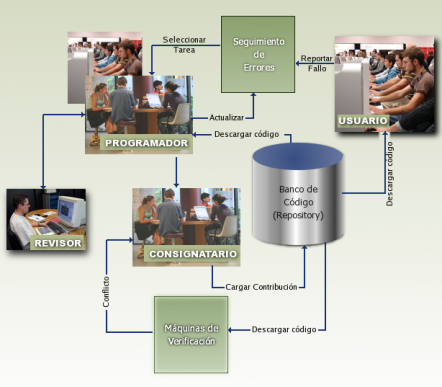
\includegraphics[width=100mm]{proceso_fs.png}
 \caption{Conceptos Básicos en el Desarrollo de Software de Código Abierto}
\label{proceso_fs} 
\end{figure}

Más que una forma de realizar sistemas, se trata de una visión revolucionaria en torno al software como patrimonio de la humanidad y se une a la filosofía del software libre que se expresa en \cite{stallman2002}:

\begin{quote}
“Software Libre” se refiere a la libertad de los usuarios para ejecutar, copiar, distribuir, estudiar, cambiar y mejorar el software. De modo más preciso, se refiere a cuatro libertades de los usuarios del software:

\begin{itemize}
\item La libertad de usar el programa, con cualquier propósito (libertad 0).
\item La libertad de estudiar cómo funciona el programa, y adaptarlo a tus necesidades (libertad 1). El acceso al código fuente es una condición previa para esto.
\item La libertad de distribuir copias, con lo que puedes ayudar a tu vecino (libertad 2).
\item La libertad de mejorar el programa y hacer públicas las mejoras a los demás, de modo que toda la comunidad se beneficie. (libertad 3). El acceso al código fuente es un requisito previo para esto.
\end{itemize}
\end{quote} 

Las aplicaciones más representativas del mundo del software libre como Apache, Mozilla, MySQL, PostgreSQL y el mismo sistema operativo Linux, luego de sus etapas primarias, adoptaron como proceso de desarrollo uno que contravenía en gran manera los fundamentos del control riguroso y ponía el futuro del sistema en manos de la anarquía \footnote{Definida en su sentido positivo como la situación humana en donde es innecesaria e indeseable la autoridad, lo que conlleva a una sociedad libre basada en el respeto mutuo de sus miembros y la cooperación voluntaria entre individuos.\cite{bce}}. Tal como lo propone Linus Torval “la idea es liberar versiones de prueba rápido a menudo, delegar cuanto sea posible, estar abierto hasta el punto de resultar promiscuo”.

Algunos principios fundamentales en este tipo de desarrollo los expone \cite{raymond}:

\begin{quote}
\begin{enumerate}
\item Todo buen trabajo de software comienza a partir de las necesidades personales del programador. (Todo buen trabajo empieza cuando uno tiene que rascarse su propia comezón). 

Esto podría sonar muy obvio: el viejo proverbio dice que "la necesidad es la madre de todos los inventos". Empero, hay muchos programadores de software que gastan sus días, a cambio de un salario, en programas que ni necesitan ni quieren. No ocurre lo mismo en el mundo Linux; lo que sirve para explicar por qué se da una calidad promedio de software tan alta en esa comunidad.
\item Los buenos programadores saben qué escribir. Los mejores, qué reescribir (y reutilizar).

... una importante característica de los grandes programadores es la meticulosidad con la que construyen. Saben que les pondrán diez no por el esfuerzo, sino por los resultados; y que casi siempre será más fácil partir de una buena solución parcial que de cero.
\item "Contemple desecharlo; de todos modos tendrá que hacerlo." cita encontrada en el capítulo 11 de libro The Mythical Man-Month escrito por el célebre Fred Brooks.

Diciéndolo de otro modo: no se entiende cabalmente un problema hasta que se implementa la primera solución. La siguiente vez quizás uno ya sepa lo suficiente para solucionarlo. Así que si quieres resolverlo, prepárate a empezar de nuevo al menos una vez.

\item Si tienes la actitud adecuada, encontrarás problemas interesantes.

\item Cuando se pierde el interés en un programa, el último deber es heredarlo a un sucesor competente.

\item. Tratar a los usuarios como colaboradores es la forma más apropiada de mejorar el código, y la más efectiva de depurarlo.

\item Libere rápido y a menudo, y escuche a sus clientes.

\item Dada una base suficiente de desarrolladores asistentes y beta-testers, casi cualquier problema puede ser caracterizado rápidamente, y su solución ser obvia al menos para alguien.

Dicho de manera menos formal, "con muchas miradas, todos los errores saltarán a la vista". A esto lo he bautizado como la Ley de Linus.

\item Las estructuras de datos inteligentes y el código burdo funcionan mucho mejor que en el caso inverso.

De nuevo Fred Brooks, Capítulo 11: “Muéstreme su código y esconda sus estructuras de datos, y continuaré intrigado. Muéstreme sus estructuras de datos y generalmente no necesitaré ver su código; resultará evidente.” 

\end{enumerate}
\end{quote} 
 
En general un proceso de desarrollo de software libre se basa en el hecho de que el programa puede ser instalado y el código fuente está disponible para cualquier persona. Es decir, la ausencia de barreras en cuanto a la limitación en el uso hace que muchas personas interesas en la funcionalidad que brinda el software lo descarguen y empiecen a utilizarlo. Dando inicio al siguiente ciclo:
\begin{enumerate}
\item El grupo inicial de programadores mantiene un sitio en la red para obtener retroalimentación de los usuarios los cuales reportan fallos, disafuncionalidades y solicitan nuevas características. 

\item Un desarrollador - que puede ser uno de los usuarios, revisa la lista de reportes y decide trabajar en uno específico; para tal efecto descarga la última versión del código fuente la modifica y la envía a un revisor para que este convalide la contribución.

\item La contribución se agrega al código fuente generando una nueva versión del sistema. Esto se realiza sincronizando el código fuente de desarrollo con aquél existente en la bodega de código fuente - repository, la cuál normalmente es un gestionada por un programa para el control de versiones. 

\item Si en algún momento dos programadores están realizando modificaciones a la misma porción de código y pretenden sincronizarlas ocurre un conflicto que deberá ser resuelto siguiendo reglas definidas que habitualmente contemplan el bloqueo de la versión más reciente, el aviso para resolución entre desarrolladores que causan el conflicto o el descarte de las contribuciones.
\end{enumerate}

De esta forma se va refinando el software siguiendo el ciclo mostrado en la figura \ref{proceso_fs}. El grupo de desarrollo se ve aumentado cuando usuarios expertos empiezan a proponer y realizar cambios directos en el código; cuando uno de ellos demuestra tener el suficiente interés y respeto hacia los intereses del software se le asigna el permiso para escribir directamente en la bodega de código.

La creación de la documentación así como de los modelos de requerimientos,análisis, diseño y despliegue siguen el mismo proceso.

\subsubsection{Métodos Ligeros}

Ha principios del milenio un grupo de experimentados desarrolladores, entre los que se encontraban Kent Beck, Alistair Cockburn, Martin Fowler y Dave Thomas, redactaron un manifiesto en el que consignaban los elementos de mayor importancia dentro del desarrollo de sistemas software \cite{beck1999}:
\begin{quote}
Nosotros estamos descubriendo mejores formas de desarrollar software dado que lo creamos y ayudamos a otros a realizar esta tarea. Por medio del trabajo de desarrollo hemos encontrado de gran valor elegir:

\begin{itemize}
\item \textbf{\textit{Individuos e interacciones}} sobre \textit{procesos y herramientas}
\item \textbf{\textit{Software ejecutable}} sobre \textit{documentación profusa}
\item \textbf{\textit{Colaboración del Cliente en el desarrollo}} sobre \textit{contrato de negocios}
\item \textbf{\textit{Respuesta al cambio}} sobre \textit{ceñirse a un plan.}
\end{itemize}

Mientras que existe valor en los elementos de la derecha nosotros valoramos más los elementos de la izquierda.\end{quote}

Con esto sentaban las bases para el despliegue de nuevos métodos de realizar software agrupados bajo el nombre genérico de “ágiles”\footnote{Siendo por definición un método caracterizado por ser liviano y ligero} que se contraponían a los métodos y procesos tradicionalmente rígidos y altamente planificados.

En \cite{koch} se expresan claramente las razones del porqué se desarrollan estos métodos y sus principales características. Los métodos ágiles nacen como respuesta del desarrollador puro al ambiente altamente industrializado y burocrático en el cual transcurren la mayoría de proyectos de desarrollo de software. En estos ambientes es típico el riguroso control que sobre el cumplimiento de cronogramas, planes de trabajo y presupuestos mantienen los denominados \textit{ingenieros de proceso}. El enfoque tradicional se basa en la planificación con la que se trata de \textit{predecir} desde las primeras etapas todos los pormenores del ciclo de desarrollo.

Debido a que los métodos tradicionales tienen fundamento en la ingeniería civil y mecánica, tratan de mitigar los riesgos poniendo un especial interés a las actividades de modelo en especial en las etapas de análisis y diseño; en general relegan a los desarrolladores a etapas de construcción erroneamente consideradas de \textit{cero esfuerzo} intelectual. Los requisitos del software se tratan de fijar desde los inicios del desarrollo, firmandose usualmente un contrato de aceptación de los mismos por parte del cliente. Estos métodos tradicionales siguen los lineamientos de aseguramiento de la calidad por la cual los procesos son eficientemente documentados, controlados, auditados, vigilados y mejorados. Todos esos aspectos hacen que el elemento clave sea el proceso y se relegue a segundo plano el crear productos que en realidad aporten un nuevo valor al cliente.

Para atacar la abrumadora complejidad que añade el proceso al sistema de software, los métodos ágiles proponen cambiar el paradigma \textit{predictivo} - rígido y resistente al cambio; por uno adaptativo que sea flexible y reaccione rápidamente antes cambios inesperados en los requisitos del software. Aquellos que han desarrollado un software de mediana o alta complejidad conocen de primera mano el hecho de que los requisitos no son estáticos, ellos cambian, evolucionan se transforman ya que en sí, no son sino abstracciones de necesidades del mundo real y este no es estático sino que se caracteriza por una fuerte dinámica.

El \textit{cliente también debe ser adaptable} en el sentido de que la mayoría de las veces los requerimientos del sistema los va descubriendo a medida que interactua con él. Una de las premisas de los procesos ágiles es el mantener un contacto permanente con el cliente e involucrarlo en todas las fases del desarrollo. Con esto se logra que el cliente obtenga un software que realmente cope sus intereses y (el cliente) sea consiente de los costos asociados al desarrollo del mismo.

Así como los requisitos cambian durante el desarrollo también lo hacen los recursos y el escenario en el cual se desenvuelve el equipo de trabajo. Para atacar esta característica de los sistemas software, se recomienda \textit{aferrarse a un presupuesto global} pero distribuyéndolo en pequeños presupuestos que solventen las tareas que ha corto plazo realizan los involucrados en el desarrollo.

Es claro con lo expuesto hasta ahora que el enfoque es considerar el desarrollo como una “\textit{carrera de 100 metros planos}” y no como una maratón. En tal sentido se deben gestar planes a corto plazo cuyo objetivo principal sea generar versiones del sistema que puedan ser probadas, corregidas e incrementalmente adicionadas en funcionalidad. Cada plan transcurre en lo que se denomina una iteración la cual usualmente no supera el mes de duración - algunos recomiendan una duración de dos semanas o ménos.\cite{beck1999}

Otro característica de los métodos clásicos, y que atacan los métodos ágiles, es aquella en la cual se considera a las personas como recursos intercambiables mediante la definición de \textit{roles} con funciones específicas y predictivas. Esto hace que las personas - cuyo comportamiento es poco predecible y no lineal \cite{cockburn1999}, tengan una moral baja y descienda su productividad; en el mejor de los casos trabajan con esfuerzo y, si sus condiciones son excelsas, rapidamente abandonan el grupo perdiéndose un activo intangible que repercute negativamente en la calidad global del sistema. Para los metodólogos ágiles el desarrollo se centra en las personas más que en los procesos, considera a cada miembro del grupo como un \textit{ser creativo e irreemplazable}, esto genera un gran cambio en cuanto al método: \textit{no es estático} ni recetario. Evoluciona, se recrea, se adapta y se concerta dentro el grupo de trabajo.

Evidentemente el proceso de desarrollo de software libre maneja los principios promulgados por los métodos ágiles los cuales encuentran quizás su máxima expresión en la Programación Extrema \cite{beck1999}.


\subsubsection{Proceso Unificado}
Según lo expresa \cite{alhir2003}:
\begin{quote}
El Proceso Unificado (UP) es un proceso de desarrollo de software basado en componentes dirigido por casos de uso, centrado en la arquitectura, iterativo e incremental...que utiliza la especificación UML dada por el Object Management Group (OMG) para preparar los esquemas del sistema. El Proceso Unificado es aplicable a diferentes tipos de sistemas de software, incluyendo proyectos de pequeña y larga escala; proyectos que tengan varios grados de complejidad técnica y administrativa, a través de diferentes dominios de aplicación y culturas organizacionales.

El PU nace de la unificación, en 1995, de la aproximación sugerida por Rational Software Corporation y el proceso orientado a objetos de la empresa Objetory AB. Se puede considerar al Proceso Unificado como un modelo de ciclo de vida del proyecto que incluye contexto, colaboraciones e interacciones. El UP es documentado totalmente en el libro “The Unified Software Development Process” escrito por Booch, Rumbaugh y Jacobson, y publicado por Addison- Wesley en 1999.\end{quote} 

Un sistema desde que nace hasta que muere repite el Proceso Unificado en ciclos de desarrollo constituidos por fases secuenciales cuyo objetivo es la producción incremental de liberaciones del sistema, llamadas comúnmente como generaciones del sistema. Cada una de las fases se convierte en un hito principal y esta constituido por pequeños microprocesos denominados \textit{iteraciones}. Habitualmente la numeración de las fases se hace de acuerdo a números enteros mientras que las iteraciones se hacen en números decimales. 

Las fases para el desarrollo de proyectos en el Proceso Unificado son cuatro \cite{jacobson2000}, a saber:

\begin{description}
\item [Fase de Concepción.] Tambien conocida como de inicio. Se centra en el establecimiento de las fronteras, ámbitos, riesgos asociados y visión del proyecto. Determina la viabilidad y los objetivos del proyecto. En esta fase podría tenerse una arquitectura general del sistema que esboze los subsistemas más importantes.

\item [Fase de Elaboración.] Se enfoca en la determinación de la arquitectura y requisitos del sistema; de esta forma se establece su viabilidad técnica. Durante esta fase se construyen los casos de uso críticos y se obtiene una arquitectura refinada del sistema. 

\item [Fase de Construcción] Es en la que se crea la mayor funcionalidad del producto, finaliza con cierta capacidad operativa. Se centra en la construcción del sistema y la arquitectura del sistema se considera estable.

\item [Fase de Transición]. Concluye con la liberación del producto, centrándose en la transición o distribución del sistema a la comunidad o usuario final. 

\end{description}

Dentro de las iteraciones el grupo de trabajo deberá distribuir sus esfuerzos en áreas estratégicas que conduzcan a la mitigación temprana de los riesgos, estás áreas son conocidas dentro del PU como disciplinas, figura \ref{proceso_unificado}:

\begin{itemize}
\item \textbf{Disciplina de administración de cambios en la configuración}, la cual se centra en la administración de la configuración del sistema y de las peticiones de cambios en la misma.

\item \textbf{Disciplina de administración de proyecto.}

\item \textbf{Disciplina de ambiente} que se centra en los ambientes de desarrollo del proyecto, incluyendo los procesos y las herramientas.

\item \textbf{Disciplina de modelado del negocio;} focalizado en la comprensión del negocio que esta siendo automatizado por el sistema capturando dicho conocimiento en un modelo del negocio.

\item \textbf{Disciplina de requerimientos,} necesaria para entender los requerimientos del sistema que automatiza el negocio y captura dichos requerimientos en un modelo de casos de uso.

\item \textbf{Disciplina de diseño y análisis,} centrada en analizar los requisitos y diseñar en sistema capturando tales  conocimientos en un modelo de análisis/diseño.

\item \textbf{Disciplina de implementación} para la implementación del sistema basado en el modelo de implementación.

\item \textbf{Disciplina de pruebas} que maneja las pruebas (evaluaciones) del sistema comparándolos con los requerimientos basándose primordialmente en el modelo de pruebas.

\item \textbf{Disciplina de distribución} encargada de la distribución del sistema basado en el modelo de distribución.
\end{itemize}

Durante la etapa de concepción la mayoría del esfuerzo está distribuido a través del modelo del negocio y la disciplina de requerimientos. 

Durante la fase de elaboración el esfuerzo se distribuye entre las disciplinas de implementación, diseño, análisis y requerimientos. Durante la etapa de construcción el esfuerzo se distribuye entre las disciplinas de análisis, diseño, implementación y pruebas. 

En la fase de transición el esfuerzo se distribuye a través de las disciplinas de prueba y distribución. Obviamente las disciplinas de soporte se distribuyen entre todas las cuatro fases. El objetivo general es producir el sistema, por lo tanto todas las disciplinas nucleares están comprometidas tanto como sea posible para no introducir riesgos en el proceso; esto es, los practicantes son los responsables de determinar cuales disciplinas comprometer y en que momento hacerlo.

En este punto es necesario definir varios conceptos: 
\begin{itemize}
\item \textbf{riesgo} en el Proceso Unificado se concibe como un obstáculo para alcanzar el éxito en la ejecución de una actividad, este riesgo puede estar determinado por características del negocio, humanas o técnicas.

\item \textbf{Iteración} es un paso o rama a través de un ruta hasta cierto destino. Dicho de otra forma es un movimiento planeado que puede ser evaluado para demostrar un progreso tangible dentro de una actividad o proceso, además, de acuerdo a lo citado por \cite{Zavala2000}: “Una iteración es iterativa en el aspecto de que es un acto repetitivo que propende la mejora continua del trabajo. Aditiva en el caso de que el resultado es siempre superior al alcanzado con un solo trabajo y paralela ya que el trabajo puede ser concurrente dentro de la iteración.”

\end{itemize}


\begin{figure}
 \centering
 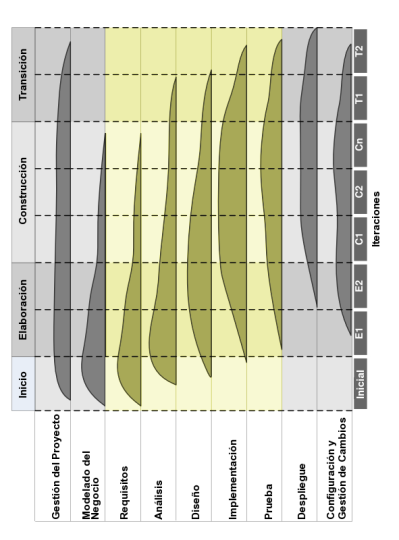
\includegraphics[width=140mm, height=190mm]{pu.png}
 \caption{Ciclo de Desarrollo de un sistema según el Proceso Unificado}
 \label{proceso_unificado}
\end{figure}

Cuando se decantan los \textit{requerimientos}, aquello que el sistema debe cumplir, se está declarando explícitamente los casos de uso los cuales, dado que el Proceso Unificado está manejado por ellos, determinan las iteraciones. De la misma forma en que los casos evolucionan en el marco de las disciplinas regidas por un proceso iterativo, los sistemas evolucionan constantemente con base en iteraciones realizados en el marco de su arquitectura. Incluyendo en la arquitectura todos los elementos, sus colaboraciones e interacciones.  

Resulta pues obvio que la iteración, dado que es un avance demostrable, tiende en últimas a reducir los riesgos inherentes a cada una de las etapas del proceso de desarrollo. Esto ha sido definido por \cite{alhir2003} en su artículo:
\begin{quote}
.. de esta forma las iteraciones confrontan los riesgos derivados de los casos de uso y la arquitectura para alcanzar el éxito en el proyecto, buscando en todo momento reconciliar las fuerza técnicas y del negocio. Una iteración esta acotada en el tiempo con inicio y final fijos en donde una colección de colaboraciones son planeadas, ejecutadas y evaluadas del tal forma que en todo momento se pueda demostrar progreso en el proceso... un caso de uso evoluciona a través de un gran número de iteraciones y a través de cualquier número de disciplinas nucleares en una iteración. La experiencia y aprendizaje obtenido en una iteración evidentemente conduce la aplicación de las próximas iteraciones dentro del proceso..\end{quote} 

La iteración se convierte en el hito más importante para asegurar el crecimiento continuo y el aseguramiento de la calidad total dentro del sistema que se está desarrollando. Las iteraciones marcan totalmente el ciclo de desarrollo del SITEM que utiliza una aproximación iterativa propuesta por el Proceso Unificado.

\section{UML: Lenguaje de Modelado Unificado}

Independiente del modelo utilizado para la construcción y gestión del desarrollo del sistema se requiere que la comunicación entre los diferentes integrantes del grupo de desarrollo sea efectiva. Se hace indispensable que todo el equipo utilice y entienda un lenguaje consistente y unificado con el cual expresen claramente sus ideas y desde el cual puedan marcar claramente las directrices a seguir. El lenguaje de Modelado Unificado, UML por sus siglas en inglés, brinda las características tanto sintácticas como semánticas para lograr caracterizar lógicamente cualquier tipo de software permitiendo ser utilizado en cualquier etapa del diseño y es especialmente útil en aquellos desarrollos enfocados a objetos.

El Lenguaje de Modelado Unificado es definido por el \textit{Object Management Group}\footnote{La página del OMG (www.omg.org) describe la organización como un consorcio de la industria de la informática, sin ánimo de lucro, con caracter internacional y de membresía abierta. Los diferentes grupos de trabajo del OMG desarrollan estándares en un rango amplio de tecnologías.}:
\begin{quote}
UML es un lenguaje visual para la especificación, construcción, y documentación de los artefactos de un sistema. Es un lenguaje de modelado de propósito generalque puede ser usado con la mayoría de los métodos orientados a objetos y a componentes; que puede ser aplicado a todos los dominios de aplicación (p.e., salud, finanzas, telecomunicaciones, aeroespacial) y plataformas de implementación (p.e., J2EE, .NET). \end{quote} 

En \cite{jacobson2005} se recalca que UML es usado para entender, diseñar, buscar, configurar, mantener y controlar la información acerca de los sistemas.

Con UML se crean artefactos con información acerca de la estructura - o vista estática- y el comportamiento - o vista dinámica- de un sistema. Cada vista del sistema se modela como una colección de objetos que interactuan, es decir, que tienen interfaces y relaciones entre ellos perfectamente definidas. Fruto de tal relación entre objetos el sistema ofrece una funcionalidad o cumple un objetivo que es de interés.